\documentclass[border=4pt]{standalone}
\usepackage[T1]{fontenc}
\usepackage{helvet}
\renewcommand{\familydefault}{\sfdefault}
\usepackage{graphicx}
\usepackage{caption}
\usepackage{amsmath}
\captionsetup{font={sf,footnotesize},labelfont={sf,bf,footnotesize},justification=justified,singlelinecheck=false}
\begin{document}
\setcounter{figure}{5}
\begin{minipage}{7.20in}
\centering
\begin{figure}[htbp]
    \centering
    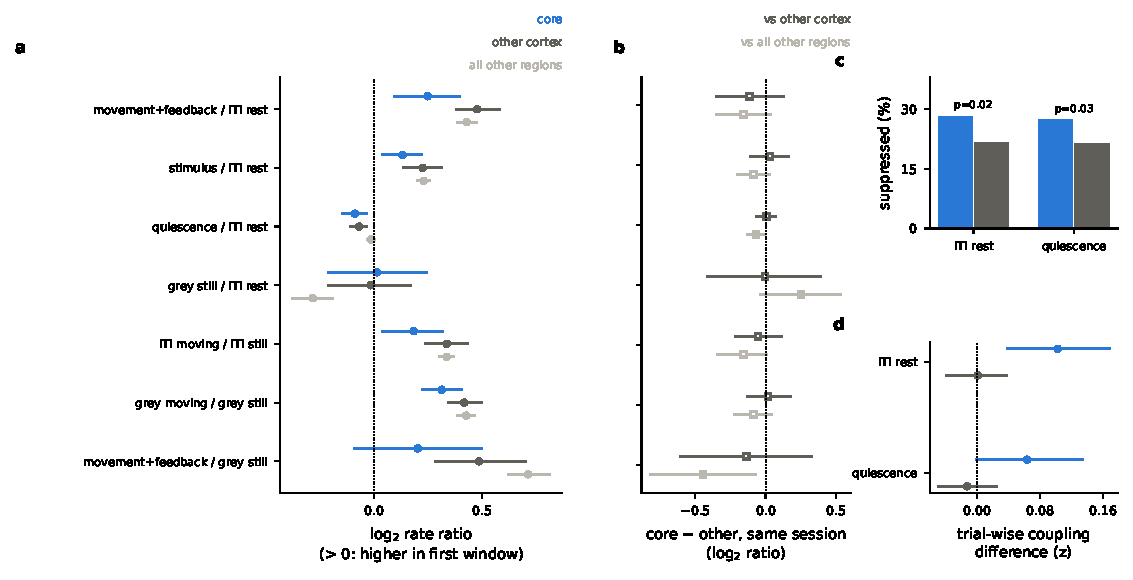
\includegraphics[width=\linewidth]{fig6_contrasts_panels.pdf}
    \caption{\textbf{a} DMN-motivated contrasts, per neuron log$_2$ ratio of session-averaged rates (+0.1 Hz), mean over mice with 95\% bootstrap CI, for the conservative core, all other cortex and all other recorded regions. A task-negative region should be below zero in the first three rows; the quiescence row separates engagement from movement, the movement rows separate movement from the task. \textbf{b} The most conservative version: core neurons minus non-core neurons recorded in the same session, averaged per mouse (31 mice vs other cortex, 49 vs all other regions); filled markers, Wilcoxon p $<$ 0.05 over mice. \textbf{c} Fraction of neurons suppressed during movement + feedback relative to ITI rest or quiescence (per-trial Welch test, p $<$ 0.01), core vs other cortex; region-permutation p. \textbf{d} Trial-by-trial co-fluctuation of region signals in ITI rest and quiescence windows (distance and probe residual; 39 core-core pairs, 26 mice): core-core minus core-other (blue) and core-other minus other-other (grey), 95\% mouse-bootstrap CI. The core-core excess comes from same-probe neighbours ($<$0.5 mm, mainly RSPd--RSPv); distance-matched within session it is +0.06 (CI $-$0.02 to 0.13).}
    \label{fig:grey_contrasts}
\end{figure}
\end{minipage}
\end{document}
